\documentclass[12pt,letterpaper]{article}
\usepackage[utf8]{inputenc}

% Ajustamos los márgenes para corregir las advertencias de fancyhdr
\usepackage[letterpaper, margin=1in, bottom=3in, top=2.2in]{geometry}

% Cargamos primero el paquete fancyhdr
\usepackage{fancyhdr}
% Corregimos los parámetros headheight y footskip
\setlength{\headheight}{15pt} % Al menos 14.49998pt según la advertencia
\setlength{\footskip}{72pt}   % Al menos 71.60547pt según la advertencia

\usepackage{xcolor}
\usepackage{amsmath}
\usepackage{anyfontsize}
\usepackage{graphicx}
\usepackage{tikz} % Necesario para los elementos gráficos
\usepackage{listings} % Para resaltado de sintaxis
\usepackage{sourcesanspro}
\renewcommand{\familydefault}{\sfdefault}
\usepackage{fontawesome5}
\usepackage{titlesec}
\usepackage{setspace}
\usepackage{hyperref}
\usepackage{mdframed} % Para marcos más estables
\usepackage{qrcode} % Paquete para generar códigos QR
\usepackage{eso-pic}

% Cargar tikz y la biblioteca de cajitas para mdframed
\usetikzlibrary{calc,shapes,positioning}

% IMPORTANT: Force the text color to be white for the entire document
\AtBeginDocument{\color{primaryColor}}

% Colors updated with better contrast
\definecolor{myblue}{cmyk}{1.0,0.8,0.05,0.20}
\definecolor{bgColor}{RGB}{15, 22, 36}  % Very dark blue, almost black background
\definecolor{primaryColor}{RGB}{255, 255, 255}  % White text - full white for better contrast
\definecolor{accentColor}{RGB}{255, 212, 59}  % Python Yellow
\definecolor{pythonBlue}{RGB}{120, 180, 255}  % Azul Python más claro para mejor contraste
\definecolor{secondaryColor}{RGB}{220, 230, 240}  % Lighter blue-gray for better contrast
\definecolor{terminalBg}{RGB}{22, 22, 22}  % Terminal background remains dark
\definecolor{terminalFrame}{RGB}{40, 40, 40}  % Terminal frame slightly darker
\definecolor{lineNumberColor}{RGB}{100, 100, 100}  % Color más sutil para los números de línea
\definecolor{dividerColor}{RGB}{60, 70, 90}  % Color más sutil para la línea divisoria

% Colores mejorados para el código con mayor contraste
\definecolor{codeTextColor}{RGB}{255, 255, 255}  % Blanco puro para el texto básico
\definecolor{codeKeywordColor}{RGB}{135, 206, 250}  % Azul cielo para palabras clave
\definecolor{codeCommentColor}{RGB}{144, 238, 144}  % Verde claro para comentarios
\definecolor{codeStringColor}{RGB}{255, 215, 135}  % Amarillo para strings
\definecolor{codeMethodColor}{RGB}{255, 160, 122}  % Naranja claro para métodos
\definecolor{codeFunctionColor}{RGB}{255, 215, 0}  % Dorado para funciones
\definecolor{codeNumberColor}{RGB}{255, 255, 150}  % Amarillo claro para números

% Set page background color
\pagecolor{bgColor}

% Hyperref configuration
\hypersetup{
    colorlinks=true,
    linkcolor=accentColor,
    filecolor=accentColor,
    urlcolor=accentColor,
}

% Configuración básica para listings que evita problemas con saltos de página
\lstset{
  language=Python,
  basicstyle=\normalsize\ttfamily\bfseries\color{codeTextColor}, % Tamaño reducido, en blanco y negrita
  backgroundcolor=\color{terminalBg},
  commentstyle=\color{codeCommentColor},
  keywordstyle=\color{codeKeywordColor},
  stringstyle=\color{codeStringColor},
  numberstyle=\color{lineNumberColor}, % Números de línea más sutiles
  breaklines=true,
  breakatwhitespace=true,
  tabsize=4,
  showstringspaces=false,
  frame=none,
  xleftmargin=15pt,
  xrightmargin=0pt,
  aboveskip=10pt,
  belowskip=10pt,
  numbers=left,
  numbersep=8pt,
  extendedchars=true,
  keepspaces=true,
  columns=flexible,
  lineskip=6pt, % Espacio entre líneas ligeramente reducido
  % Keywords de Python (palabras reservadas)
  morekeywords={self, yield, lambda, with, as, from, True, False, None, import, in, for, 
                if, elif, else, while, return, def, class, try, except, finally, raise, 
                break, continue, global, nonlocal, pass, assert, del, yield from},
  % Funciones incorporadas resaltadas de manera distinta
  emph={[2]print,range,sum,int,str,float,list,dict,set,tuple,next,len,type,map,filter,
         reduce,zip,enumerate,sorted,reversed,min,max,open,any,all},
  emphstyle={[2]\color{codeFunctionColor}}
}

% TERMINAL ESTILO MAC MEJORADA CON BOTONES A LA IZQUIERDA Y MENOS ESPACIO SUPERIOR
\newenvironment{macterminal}{%
    \begin{mdframed}[
        linecolor=terminalFrame,
        backgroundcolor=terminalBg,
        roundcorner=5pt,
        skipabove=10pt,
        skipbelow=10pt,
        linewidth=1pt,
        innertopmargin=10pt, % Reducido
        frametitle={%
            \tikz[baseline=(current bounding box.east), outer sep=0pt]{
                \fill[red!80!black] (0,0) circle (5pt);
                \fill[yellow!80!black] (0.7,0) circle (5pt);
                \fill[green!70!black] (1.4,0) circle (5pt);
            }
        },
        frametitlealignment=\raggedright, % Alineado a la izquierda
        frametitleaboveskip=8pt, % Espacio entre el título y el borde superior
        frametitlebelowskip=0pt, % Reducir el espacio entre el título y el contenido
    ]
    % No necesitamos más espacio vertical aquí
}{%
    \end{mdframed}%
}

% Utilities
\newcommand{\verspace}{\vspace{10pt}}

% Section styling - Esquema más elegante y mejorado contraste
\titleformat{\section}
  {\LARGE\bfseries\color{primaryColor}} % Secciones principales en blanco para mejor contraste y más grandes
  {\thesection. }
  {0pt}
  {}
  []

\titleformat{\subsection}
  {\Large\bfseries\color{accentColor}} % Subsecciones en amarillo Python y más grandes
  {\thesubsection. }
  {0pt}
  {}
  []

\titleformat{\subsubsection}
  {\large\bfseries\color{pythonBlue}} % Subsubsecciones en azul Python más claro y más grandes
  {\thesubsubsection. }
  {0pt}
  {}
  []

% Spacing for sections
\titlespacing*{\section}{0pt}{20pt}{10pt}
\titlespacing*{\subsection}{0pt}{15pt}{7pt}
\titlespacing*{\subsubsection}{0pt}{10pt}{5pt}

% Configure header and footer
\pagestyle{fancy}
\fancyhf{}

% Crear un encabezado elegante para todas las páginas (excepto la portada)
\fancyhead[L]{
    
\begin{tikzpicture}[remember picture, overlay]
        % Rectángulo de fondo para la sección Python
        \fill[pythonBlue, rounded corners=3pt] (0,0) rectangle (2.2cm,0.7cm);
        % Texto Python
        \node[text=primaryColor, font=\bfseries] at (1.1cm,0.35cm) {PYTHON};
        
        % Pequeño separador
        \fill[secondaryColor] (2.35cm,0.1cm) rectangle (2.40cm,0.6cm);
        
        % Texto Generators con el color de acento
        \node[text=accentColor, font=\bfseries, anchor=west] at (2.35cm,0.35cm) {GENERATORS};
    \end{tikzpicture}
}

% Línea de encabezado
\renewcommand{\headrulewidth}{0pt}

% Configure footer with profile info
\fancyfoot[C]{
    \vspace*{0.2cm}
    \noindent
    \begin{minipage}{\textwidth}
        \begin{flushleft}
            % Profile image placeholder with TikZ
            \raisebox{0.7cm}{
            \begin{tikzpicture}[baseline]
                \path[fill=bgColor] (0,0) circle (0.8cm);
                \clip (0,0) circle (0.8cm);
                \node at (0,0) {
                    % Placeholder for profile image
                    \includegraphics[width=1.6cm,height=1.6cm]{slides/profile-image.jpeg}
                };
            \end{tikzpicture}
            }
            \begin{minipage}[b]{0.8\textwidth}
                % Name
                {\large\bfseries\color{primaryColor}Alejandro Sánchez Yalí}
                
                % Professional description
                \par\vspace{1pt}
                {\small\color{secondaryColor}Software Developer | AI \& Blockchain Enthusiast}
                
                % Contact
                \par\vspace{1pt}
                {\small\color{accentColor}\faGlobe\hspace{5pt}\color{secondaryColor}www.asanchezyali.com}
            \end{minipage}
        \end{flushleft}
        \vspace{8pt} % Space at bottom
    \end{minipage}
}

% Estilo para la portada (sin encabezado ni pie de página)
\fancypagestyle{plain}{
    \fancyhf{}
    \renewcommand{\headrulewidth}{0pt}
    \renewcommand{\footrulewidth}{0pt}
}

% Bullet styling for lists
\renewcommand{\labelitemi}{\textcolor{accentColor}{$\bullet$}} % Primer nivel de viñetas en amarillo (mejor contraste)
\renewcommand{\labelitemii}{\textcolor{pythonBlue}{$\circ$}} % Segundo nivel de viñetas en azul

% Aumentar globalmente el tamaño de texto un 20%
\usepackage{relsize}
\AtBeginDocument{\relsize{1}} % Incrementa la fuente en aproximadamente un 20%

% Comando simplificado para la etiqueta Python
\newcommand{\languagetag}[1]{
    \begin{tikzpicture}[baseline]
        \node[fill=pythonBlue, text=primaryColor, rounded corners=5pt, inner sep=7pt] {
            {\normalsize\textbf{#1}}
        };
    \end{tikzpicture}
}


\newcommand{\BackgroundPic}{%
    \put(0,0){%
        \begin{tikzpicture}[remember picture, overlay]
            % Coloca la imagen de fondo que cubra toda la página
            \node[inner sep=0pt] at (current page.center) {
                \includegraphics[width=\paperwidth,height=\paperheight,keepaspectratio=false]{slides/Coding in Cyberpunk Style.jpeg}
            };
            
            % Agrega una capa semitransparente oscura sobre la imagen
            % Puedes ajustar el color y la opacidad según necesites
            \fill[black, opacity=0.7] (current page.south west) rectangle (current page.north east);
            
            % Si quieres un degradado oscuro en lugar de un color sólido, usa esto:
            % \shade[top color=black!80, bottom color=black!40, opacity=0.7] 
            %    (current page.south west) rectangle (current page.north east);
        \end{tikzpicture}%
    }%
}

% Alternativa usando una versión modificada de la URL
\newcommand{\elegantqr}[2]{
    \qrcode[height=2.5cm]{#1}
    \\[0.1cm]
    {\hspace{0.2cm}\color{primaryColor}\small #2\par}
}

% Definir el título personalizado con alineación exacta para todos los elementos
\newcommand{\titlepagecontents}{%
    \AddToShipoutPicture*{\BackgroundPic}
    \vspace*{3cm}
    % Asegurar que todos los elementos estén alineados a la izquierda
    \begin{flushleft}
    \languagetag{Python}\\[0.4cm]
    {\fontsize{48}{52}\bfseries\color{primaryColor}Python \color{accentColor}Generators\par}
    \vspace{0.3cm}
    {\fontsize{18}{52}\color{secondaryColor}Elegant, Memory-Efficient Iterations A Powerful Python Feature\par}
    \vspace{0.3cm}
    {\color{secondaryColor}\today\par}
    \vspace{2cm}
    % El QR se alineará a la izquierda aunque internamente esté centrado
    \elegantqr{https://github.com/asanchezyali/social-media-posts/tree/main/Python/Generators}{Source Code}
    \end{flushleft}
}


% En la página del título, aplicar el contenido sin márgenes adicionales
\makeatletter
\renewcommand{\maketitle}{%
    \begin{titlepage}
    \setlength{\parindent}{0pt}
    \setlength{\leftskip}{0pt}
    \titlepagecontents
    \end{titlepage}
}
\makeatother

% También necesitamos corregir la definición para la página final
\newcommand{\finalpagecontents}{%
    \vspace*{4cm}
    \begin{center}
        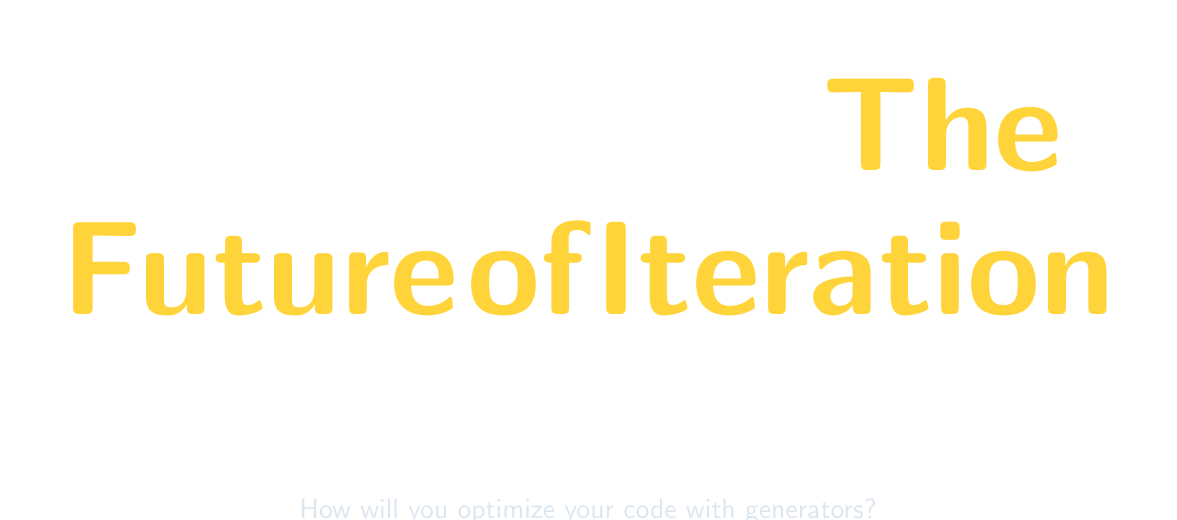
\begin{tikzpicture}
            % Title text
            \node[text width=14cm, align=center] at (0,0) {
                {\fontsize{48}{52}\bfseries\color{primaryColor}Generators: \color{accentColor}The Future of Iteration\par}
            };
            
            % Add vertical space
            \node at (0,-2) {};
            
            % Question text
            \node[text width=14cm, align=center] at (0,-4) {
                {\fontsize{22}{26}\color{secondaryColor}How will you optimize your code with generators?\par}
            };
        \end{tikzpicture}
    \end{center}
}

\begin{document}
\setlength{\parindent}{0pt}
% Eliminamos el redundante \color{primaryColor} aquí

\begin{titlepage}
    % Eliminamos todos los espacios adicionales para asegurar la alineación
    \titlepagecontents
\end{titlepage}

\section{Introduction to Python Generators}

Python generators provide an elegant way to create iterators with minimal memory footprint. Unlike lists that store all values in memory, generators produce values on-the-fly, making them ideal for handling large datasets or infinite sequences.

\subsection{What Are Generators?}

Generators are special functions that return an iterator using the \textbf{\textcolor{accentColor}{yield}} statement instead of \textbf{\textcolor{pythonBlue}{return}}. This allows the function to pause execution and later resume from where it left off.

\begin{itemize}
    \item \textbf{\textcolor{pythonBlue}{Memory Efficiency:}} Values are generated one at a time, not stored in memory
    \item \textbf{\textcolor{pythonBlue}{Lazy Evaluation:}} Values are computed only when needed
    \item \textbf{\textcolor{pythonBlue}{Simplicity:}} Cleaner code compared to implementing iterators manually
    \item \textbf{\textcolor{pythonBlue}{State Preservation:}} Generators maintain their state between calls
    \item \textbf{\textcolor{pythonBlue}{Sequence Creation:}} Easily model complex or infinite sequences
\end{itemize}

When using \textbf{\textcolor{accentColor}{yield}}, the internal state of the function (local variables and execution point) is saved, allowing the function to resume from where it left off on the next call to \texttt{next()}.

\subsection{Generators vs. Lists}

When comparing generators to traditional data structures like lists, we find several key differences:

\begin{macterminal}
\begin{lstlisting}
# List comprehension - loads all in memory
numbers_list = [x * 2 for x in range(1000000)]

# Generator expression - computes on-demand
numbers_gen = (x * 2 for x in range(1000000))

# Memory comparison
import sys
list_size = sys.getsizeof(numbers_list) 
# ~8.06 MB
gen_size = sys.getsizeof(numbers_gen)    
# ~200B
\end{lstlisting}
\end{macterminal}

Other important differences include:

\begin{itemize}
    \item \textbf{\textcolor{pythonBlue}{Memory Usage:}} Generators consume significantly less memory than equivalent lists
    \item \textbf{\textcolor{pythonBlue}{Computation:}} Lists compute all values at once; generators compute values on-demand
    \item \textbf{\textcolor{pythonBlue}{Access Patterns:}} Lists allow random access; generators only permit sequential access
    \item \textbf{\textcolor{pythonBlue}{Reusability:}} Lists can be iterated multiple times; generators are exhausted after one iteration
\end{itemize}

\section{Creating Python Generators}

There are two primary ways to create generators in Python: generator functions and generator expressions.

\subsection{Generator Functions}

Generator functions look like regular functions but use the \textbf{\textcolor{accentColor}{yield}} keyword to return values:

\begin{macterminal}
\begin{lstlisting}
def countdown(n):
    """A simple generator function that counts down from n to 1"""
    print("Starting countdown!")
    while n > 0:
        yield n
        n -= 1
    print("Countdown complete!")

# Using the generator
counter = countdown(5)
print(next(counter))  # 5
print(next(counter))  # 4
print(next(counter))  # 3
\end{lstlisting}
\end{macterminal}

The state of the function is preserved between yields, allowing it to resume execution from where it left off.

\subsection{Generator Expressions}

Generator expressions provide a concise way to create generators, similar to list comprehensions but with parentheses instead of square brackets:

\begin{macterminal}
\begin{lstlisting}
# Method 1: Generator function with yield
def count_up_to(max):
    count = 1
    while count <= max:
        yield count
        count += 1

# Method 2: Generator expression
squares = (x**2 for x in range(10))

# Using generators
for num in count_up_to(5):
    print(num)  # Prints: 1, 2, 3, 4, 5

for num in squares:
    print(num)  # Prints: 0, 1, 4, 9, 16, 25, 36, 49, 64, 81
\end{lstlisting}
\end{macterminal}

\section{Working with Python Generators}

Generators can be used in many contexts where iterables are expected.

\subsection{Basic Operations with Generators}

Here are common ways to interact with generators:

\begin{macterminal}
\begin{lstlisting}
def first_n_fibonacci(n):
    """Generate first n Fibonacci numbers"""
    a, b = 0, 1
    count = 0
    while count < n:
        yield a
        a, b = b, a + b
        count += 1

# Iterating with a for loop
fib = first_n_fibonacci(10)
for num in fib:
    print(num, end=' ')  # 0 1 1 2 3 5 8 13 21 34

# Alternatively with next()
fib = first_n_fibonacci(5)
print(next(fib))  # 0
print(next(fib))  # 1
print(next(fib))  # 1
\end{lstlisting}
\end{macterminal}

\subsection{Infinite Sequences}

Generators are particularly useful for working with potentially infinite sequences:

\begin{macterminal}
\begin{lstlisting}
# Creating an infinite sequence of Fibonacci numbers
def fibonacci():
    a, b = 0, 1
    while True:
        yield a
        a, b = b, a + b

# Using the infinite generator safely
fib_gen = fibonacci()
for _ in range(10):
    print(next(fib_gen))
    
# Output: 0, 1, 1, 2, 3, 5, 8, 13, 21, 34
\end{lstlisting}
\end{macterminal}

\subsection{The yield from Statement}

Python 3.3 introduced the \textbf{\textcolor{accentColor}{yield from}} statement, which simplifies delegation to sub-generators:

\begin{macterminal}
\begin{lstlisting}
from collections.abc import Sequence

# Without yield from
def subgenerator(n):
    for i in range(n):
        yield i

def main_generator_old(n):
    for val in subgenerator(n):
        yield val

# With yield from - more elegant
def main_generator_new(n):
    yield from subgenerator(n)
    
def flatten(nested_list):
    for item in nested_list:
        if isinstance(item, Sequence) and not isinstance(item, (str, bytes)):
            yield from flatten(item)
        else:
            yield item
\end{lstlisting}
\end{macterminal}

\section{Generator Pipelines}

Generators can be chained together to create powerful data processing pipelines:

\begin{macterminal}
\begin{lstlisting}
def read_file(file_path):
    with open(file_path, 'r') as f:
        for line in f:
            yield line.strip()

def grep(lines, pattern):
    for line in lines:
        if pattern in line:
            yield line

def uppercase(lines):
    for line in lines:
        yield line.upper()
        
# Usage
file_lines = read_file('data.txt')
filtered = grep(file_lines, 'python')
result = uppercase(filtered)

# Process results
for line in result:
    print(line)
\end{lstlisting}
\end{macterminal}

This approach is memory-efficient because each line is processed one at a time through the entire pipeline.

\section{Memory Efficiency with Generators}

One of the main advantages of generators is their memory efficiency.

\subsection{Memory Comparison: Lists vs. Generators}

Let's compare memory usage between lists and generators:

\begin{macterminal}
\begin{lstlisting}
import tracemalloc

# Start memory monitoring
tracemalloc.start()

# Create a large list
large_list = [i * i for i in range(1000000)]
list_snapshot = tracemalloc.take_snapshot()
list_size = sum(stat.size for stat in list_snapshot.statistics('filename'))

# Reset monitoring
tracemalloc.stop()
tracemalloc.start()

# Create an equivalent generator
large_gen = (i * i for i in range(1000000))
gen_snapshot = tracemalloc.take_snapshot()
gen_size = sum(stat.size for stat in gen_snapshot.statistics('filename'))

# Compare memory usage
print(f"List memory: {list_size / 1024 / 1024:.8f} MB")
print(f"Generator memory: {gen_size / 1024 / 1024:.8f} MB")
print(f"Memory ratio: {list_size / gen_size:.0f}x")

# Output:
# List memory: 38.57472229 MB
# Generator memory: 0.00038147 MB
# Memory ratio: 101121x
\end{lstlisting}
\end{macterminal}

While generators save memory, they can be slower than lists for operations requiring repeated access, as values must be recalculated each time.

\subsection{Processing Large Files}

Generators are particularly useful when working with files that would be too large to fit in memory:

\begin{macterminal}
\begin{lstlisting}
# Processing a large file with a list
def process_file_list(filename):
    with open(filename) as f:
        # All lines loaded in memory at once
        return [line.upper() for line in f]

# Processing with a generator
def process_file_generator(filename):
    with open(filename) as f:
        for line in f:
            # Process one line at a time
            yield line.upper()
\end{lstlisting}
\end{macterminal}

The memory savings can be substantial, especially when processing large datasets.

\section{The Iterator Protocol}

Under the hood, generators implement Python's iterator protocol, which requires \textbf{\textcolor{accentColor}{\_\_iter\_\_}} and \textbf{\textcolor{accentColor}{\_\_next\_\_}} methods:

\begin{macterminal}
\begin{lstlisting}
# Generator functions implement this protocol:
class Counter:
    def __init__(self, max_value):
        self.max_value = max_value
        self.current = 0
        
    def __iter__(self):
        return self
        
    def __next__(self):
        if self.current >= self.max_value:
            raise StopIteration
        self.current += 1
        return self.current

# Example usage
counter = Counter(5)
for number in counter:
    print(number) 

# Output: 1, 2, 3, 4, 5
\end{lstlisting}
\end{macterminal}

Generators eliminate the need to manually implement \texttt{\_\_iter\_\_} and \texttt{\_\_next\_\_}, as Python automatically generates them when you use \texttt{yield}.

\section{Real-World Applications}

\subsection{Log Processing}

Efficiently process large log files without excessive memory usage:

\begin{macterminal}
\begin{lstlisting}
# Processing a large log file efficiently
def parse_log_line(line):
    # Extract timestamp and message
    parts = line.split(" ", 1)
    return {"timestamp": parts[0], "message": parts[1]}

def filter_errors(log_entries):
    for entry in log_entries:
        if "ERROR" in entry["message"]:
            yield entry

def process_logs(filename):
    with open(filename) as f:
        # Parse each line
        entries = (parse_log_line(line) for line in f)
        # Filter for errors
        errors = filter_errors(entries)
        # Group by hour
        for error in errors:
            yield error
\end{lstlisting}
\end{macterminal}

\subsection{Data Transformation Pipelines}

Create efficient data processing workflows:

\begin{macterminal}
\begin{lstlisting}
def csv_reader(file_path):
    for line in open(file_path, 'r'):
        yield line.strip().split(',')

def select_columns(data, indices):
    for row in data:
        yield [row[i] for i in indices]

def filter_rows(data, condition_func):
    for row in data:
        if condition_func(row):
            yield row
            
# Usage example
data = csv_reader('large_dataset.csv')
selected = select_columns(data, [0, 2, 3])
filtered = filter_rows(selected, lambda x: float(x[1]) > 100)

for row in filtered:
    print(row)
\end{lstlisting}
\end{macterminal}

\subsection{Generators with itertools}

Combining generators with Python's itertools library provides powerful data manipulation capabilities:

\begin{macterminal}
\begin{lstlisting}
from itertools import islice

def fibonacci():
    a, b = 0, 1
    while True:
        yield a
        a, b = b, a + b

fib_slice = islice(fibonacci(), 10)
print(list(fib_slice))  # [0, 1, 1, 2, 3, 5, 8, 13, 21, 34]
\end{lstlisting}
\end{macterminal}

\section{Best Practices}

To get the most from generators in Python:

\begin{itemize}
    \item \textbf{\textcolor{pythonBlue}{Use generator expressions}} for simple transformations
    \item \textbf{\textcolor{pythonBlue}{Use generator functions}} for complex logic or when state is needed
    \item \textbf{\textcolor{pythonBlue}{Chain generators together}} to create processing pipelines
    \item \textbf{\textcolor{pythonBlue}{Remember generators are single-use}} — create new ones if needed
    \item \textbf{\textcolor{pythonBlue}{Use yield from}} to delegate to sub-generators
    \item \textbf{\textcolor{pythonBlue}{Add type hints}} with typing.Generator for clarity
    \item \textbf{\textcolor{pythonBlue}{Consider contextlib.contextmanager}} for resource management
\end{itemize}

\section{Conclusion}

Python generators provide an elegant, memory-efficient way to work with data sequences and iterative computations. They excel in scenarios involving large datasets, stream processing, and computational pipelines.

\subsection{Key Takeaways}

\begin{itemize}
    \item \textbf{\textcolor{pythonBlue}{Memory Efficiency:}} Generators calculate values on-demand, avoiding memory overhead
    \item \textbf{\textcolor{pythonBlue}{Lazy Evaluation:}} Computation happens only when needed, improving performance
    \item \textbf{\textcolor{pythonBlue}{Elegant APIs:}} Create clean, readable code for data processing pipelines
    \item \textbf{\textcolor{pythonBlue}{Infinite Sequences:}} Work with potentially infinite data without memory concerns
    \item \textbf{\textcolor{pythonBlue}{Foundation for Async:}} Generators provided the foundation for Python's async/await syntax
\end{itemize}

Mastering generators is an essential skill for writing efficient, elegant Python code, especially when dealing with large data processing tasks.

\subsection{Further Reading}

To dive deeper into Python generators, check these resources:
\begin{itemize}
    \item PEP 255 - The original Python Generator proposal
    \item \textit{Fluent Python} by Luciano Ramalho, which dedicates an entire chapter to iterators and generators
    \item Python's official documentation on generators and the itertools module
    \item Remember this document was translated, edited and written in collaboration with AI.
\end{itemize}

\section{Explore My Other Posts}
\vspace{10pt}
\begin{tikzpicture}
  % Section background - increased height slightly to ensure all content fits
  \fill[color=terminalBg, rounded corners=5pt] (0,0) rectangle (\textwidth,-5);
  
  % Calculate width available for text (total width minus QR code width minus margins)
  \pgfmathsetmacro{\availableWidth}{\textwidth-4cm}
  
  % Left column content
  \begin{scope}
    % Section title
    \node[text=accentColor, font=\Large\bfseries, anchor=north west] at (0.5cm,-0.5cm) {Enjoyed This Content?};
    
    % Subtitle
    \node[text=primaryColor, font=\normalsize, anchor=north west] at (0.5cm,-1.2cm) {Don't miss my previous post about:};
    
    % Python post title - with highlighted style and limited width
    \node[text=secondaryColor, font=\large\bfseries, anchor=north west, text width=\availableWidth] at (0.5cm,-1.9cm) {\color{accentColor}Python Context Managers: \color{primaryColor}Elegant Resource Management with the «{\color{accentColor}with}» Statement};
    
    % Brief description of the post - with limited width and adjusted position
    \node[text=secondaryColor, font=\small, text width=\availableWidth, anchor=north west] at (0.5cm,-3.1cm) {
      Discover how Python Context Managers can help you elegantly manage resources, 
      prevent memory leaks, and write cleaner code.
    };
  \end{scope}
  
  % QR Code on the right - vertically centered
  \node[anchor=center] at ({\textwidth-1.5cm}, {-2.5cm}) {
    \qrcode[height=2.5cm]{https://www.linkedin.com/feed/update/urn:li:activity:7307438566157021186/}
  };
  
\end{tikzpicture}
\vspace{5pt}

\clearpage
\thispagestyle{empty}
\finalpagecontents

\end{document}